\section{Preprocessing}

Pimpalkhute et al.~\cite{pimpalkhute2014phonetic} noted that preprocessing medication names in social media data often faces the problem of phonetic spelling. Their proposed model found that 50.4 – 56.0 \% of the user comments using only about 18\% of the variants (of spelling). The method, as shown in Figure~\ref{fig:model-pimpalkhute}, is based on the intuitive notion that people will tend to spell drug names phonetically. They have used tools and libraries such as the LOGIOS Lexicon Tool~\footnote{\url{http://www.speech.cs.cmu.edu/tools/lextool.html}}, Metaphone library~\footnote{\url{https://en.wikipedia.org/wiki/Metaphone}}, and CMU library~\footnote{\url{https://en.wikipedia.org/wiki/CMU Pronouncing Dictionary}}. The drug names are available in DrugBank~\footnote{\url{https://go.drugbank.com/stats}}. Limsopatham et al.~\cite{limsopatham2015adapting} used a phrase-based machine translation technique~\cite{koehn2003statistical} to translate phrases from ~\textit{Twitter language to formal medical language}.

\begin{figure}[h]
	\centering
	\begin{minipage}{0.45\textwidth}
		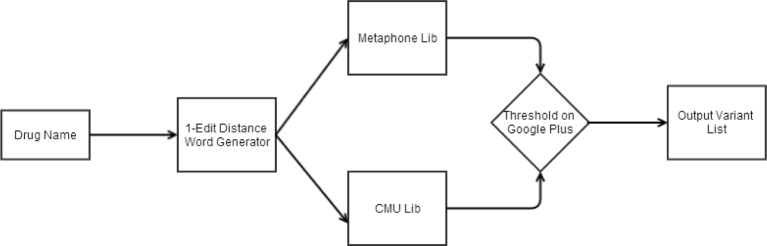
\includegraphics[width=0.99\linewidth]{Figures/m.png}
		\caption{Flow chart of Pimpalkhute et al.~\cite{pimpalkhute2014phonetic} methodology.}
		\label{fig:model-pimpalkhute}
	\end{minipage}
	\hfill
	\begin{minipage}{0.45\textwidth}
		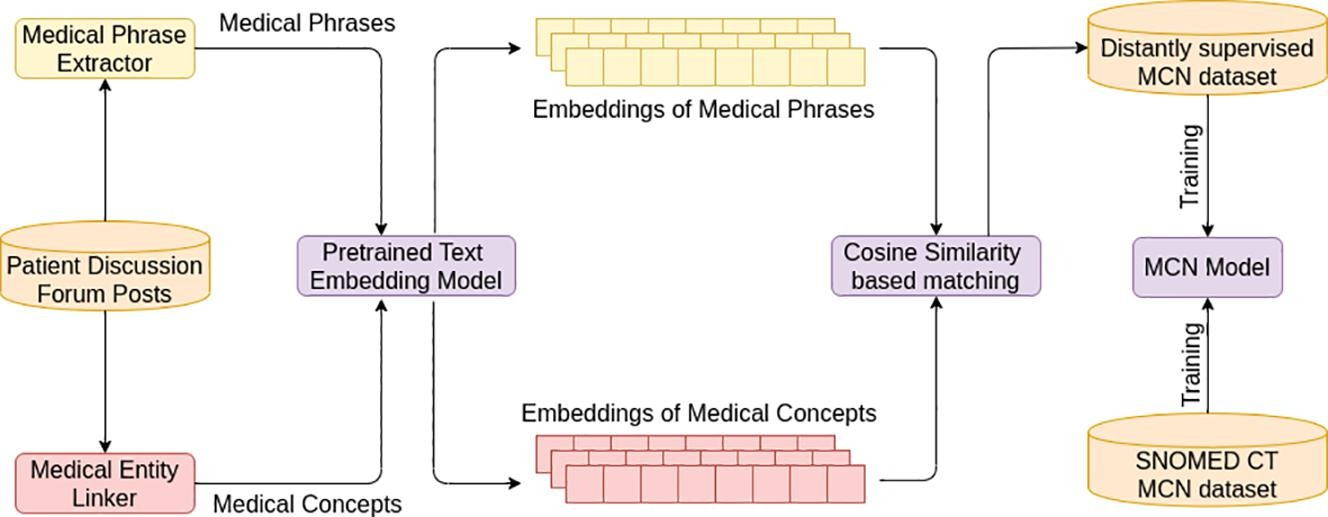
\includegraphics[width=0.99\linewidth]{Figures/o.jpg}
		\caption{Distant supervision for MCN model by Pattisapu et al.~\cite{PATTISAPU2020103522}.}
		\label{fig:medication-concept-normalization}
	\end{minipage}
\end{figure}

Limsopatham et al.~\cite{limsopatham2016normalising} later proposed two different architecture for medical concept normalization (MCN) - a Convolutional Neural Network (CNN) model (Figure~\ref{fig:cnn-medication-concept-normalization}) and a Recurrent Neural Network (RNN) model (Figure~\ref{fig:rnn-medication-concept-normalization}). Pattisapu et al.~\cite{PATTISAPU2020103522} proposed MCN  maps to translate from informal phrases to formal medical concepts. Their proposed model is highlighted in Figure~\ref{fig:medication-concept-normalization}.


\begin{figure}[h]
	\centering
	\begin{minipage}{0.45\textwidth}
		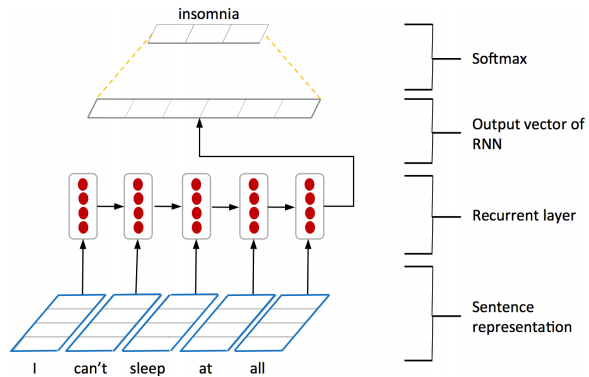
\includegraphics[width=0.99\linewidth]{Figures/q.png}
		\caption{RNN model for MCN model by Limsopatham et al.~\cite{limsopatham2016normalising}.}
		\label{fig:rnn-medication-concept-normalization}
	\end{minipage}
	\hfill
	\begin{minipage}{0.45\textwidth}
		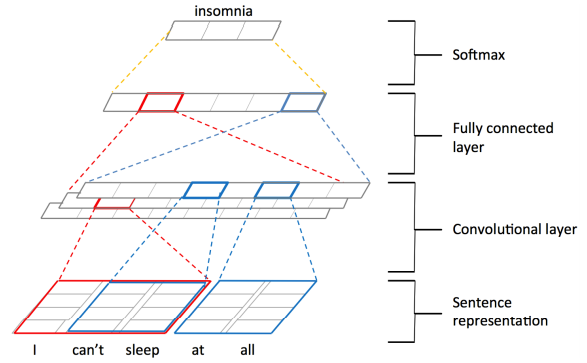
\includegraphics[width=0.99\linewidth]{Figures/p.png}
		\caption{CNN model for MCN model by Limsopatham et al.~\cite{limsopatham2016normalising}.}
		\label{fig:cnn-medication-concept-normalization}
	\end{minipage}
\end{figure}
